\documentclass[11pt]{article}
%%%%%%%%% options for the file macros.tex

\def\showauthornotes{1}
\def\showkeys{0}
\def\showdraftbox{0}
% \allowdisplaybreaks[1]

%% Shamelessly adapted from a scribe template by Sanjeev Arora

%%%%%%%%%%%%%% Packages
% \usepackage[active,tightpage]{preview}
% \renewcommand{\PreviewBorder}{1in}
\usepackage{hyperref}
\usepackage{amsmath,amssymb,amsthm,amstext,amsfonts,bbm,algorithm,algorithmicx,xspace,nicefrac,
  algpseudocode}
\usepackage{color,stmaryrd,enumerate,latexsym,bm,amsfonts,
  subfigure,wrapfig,verbatim,tabularx,textcomp}
\usepackage[small]{caption}
\usepackage{comment} 
\usepackage{epsfig} 
\usepackage{latexsym,nicefrac,bbm}
\usepackage{xspace}
\usepackage{color,fancybox,graphicx,url,subfigure}
\usepackage{enumitem, fullpage}
\usepackage{booktabs}
\usepackage{commath}
\usepackage{mdframed}
\usepackage{pdfsync}
\usepackage{tikz}
\usetikzlibrary {positioning}

%%%%%%%%%%%%%% Use for definitions
\newcommand{\defeq}{\stackrel{\textup{def}}{=}}

%%%%%%%%%%%%%% Theorem Environments
\newtheorem{theorem}{Theorem}[section]
\newtheorem{problem}[theorem]{Problem}
\newtheorem{lemma}[theorem]{Lemma}
\newtheorem{definition}[theorem]{Definition}
\newtheorem{corollary}[theorem]{Corollary}
\newtheorem{conjecture}[theorem]{Conjecture}
\newtheorem{proposition}[theorem]{Proposition}
\newtheorem{fact}[theorem]{Fact}
\newtheorem{remark}[theorem]{Remark}

%%%%%%%%%%%%%% Probability stuff
\DeclareMathOperator*{\pr}{\bf Pr}
\DeclareMathOperator*{\av}{\mathbbm{E}}
\DeclareMathOperator*{\var}{\bf Var}

%%%%%%%%%%%%%% Matrix stuff
\newcommand{\tr}[1]{\mathop{\mbox{Tr}}\left({#1}\right)}
\newcommand{\diag}[1]{{\bf Diag}\left({#1}\right)}

%% Notation for integers, natural numbers, reals, fractions, sets, cardinalities
%%and so on
\newcommand{\nfrac}[2]{\nicefrac{#1}{#2}}
\def\abs#1{\left| #1 \right|}
\renewcommand{\norm}[1]{\ensuremath{\left\lVert #1 \right\rVert}}

\newcommand{\floor}[1]{\left\lfloor\, {#1}\,\right\rfloor}
\newcommand{\ceil}[1]{\left\lceil\, {#1}\,\right\rceil}

\newcommand{\pair}[1]{\left\langle{#1}\right\rangle} %for inner product

\newcommand\B{\{0,1\}}      % boolean alphabet  use in math mode
\newcommand\bz{\mathbb Z}
\newcommand\nat{\mathbb N}
\newcommand\rea{\mathbb R}
\newcommand\com{\mathbb{C}}
\newcommand\plusminus{\{\pm 1\}}
\newcommand\Bs{\{0,1\}^*}   % B star use in math mode
\newcommand{\ones}{\mathbbm{1}}
\newcommand{\eye}{\mathbbm{I}}



\newcommand{\V}[1]{\mathbf{#1}\ignorespaces}
\renewcommand\AA{\boldsymbol{\mathit{A}}}
\newcommand\LL{\boldsymbol{\mathit{L}}}

% Used to denote bold commands
                                % e.g. vectors, matrices
\DeclareRobustCommand{\fracp}[2]{{#1 \overwithdelims()#2}}
\DeclareRobustCommand{\fracb}[2]{{#1 \overwithdelims[]#2}}
\newcommand{\marginlabel}[1]%
{\mbox{}\marginpar{\it{\raggedleft\hspace{0pt}#1}}}
\newcommand\card[1]{\left| #1 \right|} %cardinality of set S; usage \card{S}
\renewcommand\set[1]{\left\{#1\right\}} %usage \set{1,2,3,,}
\renewcommand\complement{\ensuremath{\mathsf{c}}}
\newcommand\poly{\mbox{poly}}  %usage \poly(n)
\newcommand{\comp}[1]{\overline{#1}}
\newcommand{\smallpair}[1]{\langle{#1}\rangle}
\newcommand{\ol}[1]{\ensuremath{\overline{#1}}\xspace}
\newcommand{\eps}{\epsilon}
\DeclareMathOperator{\vol}{\mathsf{vol}}


%%%%%%%%%%%%%% Mathcal shortcuts
\newcommand\calF{\mathcal{F}}
\newcommand\calP{\mathcal{P}}
\newcommand\calS{\mathcal{S}}
\newcommand\calG{\mathcal{G}}
\newcommand\calH{\mathcal{H}}
\newcommand\calC{\mathcal{C}}
\newcommand\calD{\mathcal{D}}
\newcommand\calI{\mathcal{I}}
\newcommand\calV{\mathcal{V}}
\newcommand\calK{\mathcal{K}}
\newcommand\calN{\mathcal{N}}
\newcommand\calX{\mathcal{X}}
\newcommand\calU{\mathcal{U}}
\newcommand\calE{\mathcal{E}}

%%%%%%%%%%%%%% {{{ authornotes }}}
\definecolor{Mygray}{gray}{0.8}

 \ifcsname ifcommentflag\endcsname\else
  \expandafter\let\csname ifcommentflag\expandafter\endcsname
                  \csname iffalse\endcsname
\fi

\ifnum\showauthornotes=1
\newcommand{\todo}[1]{\colorbox{Mygray}{\color{red}#1}}
\else
\newcommand{\todo}[1]{#1}
\fi

\ifnum\showauthornotes=1
\newcommand{\Authornote}[2]{{\sf\small\color{red}{[#1: #2]}}}
\newcommand{\Authoredit}[2]{{\sf\small\color{red}{[#1]}\color{blue}{#2}}}
\newcommand{\Authorcomment}[2]{{\sf \small\color{gray}{[#1: #2]}}}
\newcommand{\Authorfnote}[2]{\footnote{\color{red}{#1: #2}}}
\newcommand{\Authorfixme}[1]{\Authornote{#1}{\textbf{??}}}
\newcommand{\Authormarginmark}[1]{\marginpar{\textcolor{red}{\fbox{%\Large
#1:!}}}}
\else
\newcommand{\Authornote}[2]{}
\newcommand{\Authoredit}[2]{}
\newcommand{\Authorcomment}[2]{}
\newcommand{\Authorfnote}[2]{}
\newcommand{\Authorfixme}[1]{}
\newcommand{\Authormarginmark}[1]{}
\fi


%%%%%%%%%%%%%% Logical operators
\newcommand\true{\mbox{\sc True}}
\newcommand\false{\mbox{\sc False}}
\def\scand{\mbox{\sc and}}
\def\scor{\mbox{\sc or}}
\def\scnot{\mbox{\sc not}}
\def\scyes{\mbox{\sc yes}}
\def\scno{\mbox{\sc no}}

%% Parantheses
\newcommand{\paren}[1]{\unskip\left({#1}\right)}
\newcommand{\sqparen}[1]{\unskip\left[{#1}\right]}
\newcommand{\curlyparen}[1]{\unskip\left\{{#1}\right\}}
\newcommand{\smallparen}[1]{\unskip({#1})}
\newcommand{\smallsqparen}[1]{\unskip[{#1}]}
\newcommand{\smallcurlyparen}[1]{\unskip\{{#1}\}}

%% short-hands for relational simbols

\newcommand{\from}{:}
\newcommand\xor{\oplus}
\newcommand\bigxor{\bigoplus}
\newcommand{\logred}{\leq_{\log}}
\def\iff{\Leftrightarrow}
\def\implies{\Rightarrow}




%% macros to write pseudo-code

\newlength{\pgmtab}  %  \pgmtab is the width of each tab in the
\setlength{\pgmtab}{1em}  %  program environment
 \newenvironment{program}{\renewcommand{\baselinestretch}{1}%
\begin{tabbing}\hspace{0em}\=\hspace{0em}\=%
\hspace{\pgmtab}\=\hspace{\pgmtab}\=\hspace{\pgmtab}\=\hspace{\pgmtab}\=%
\hspace{\pgmtab}\=\hspace{\pgmtab}\=\hspace{\pgmtab}\=\hspace{\pgmtab}\=%
\+\+\kill}{\end{tabbing}\renewcommand{\baselinestretch}{\intl}}
\newcommand {\BEGIN}{{\bf begin\ }}
\newcommand {\ELSE}{{\bf else\ }}
\newcommand {\IF}{{\bf if\ }}
\newcommand {\FOR}{{\bf for\ }}
\newcommand {\TO}{{\bf to\ }}
\newcommand {\DO}{{\bf do\ }}
\newcommand {\WHILE}{{\bf while\ }}
\newcommand {\ACCEPT}{{\bf accept}}
\newcommand {\REJECT}{\mbox{\bf reject}}
\newcommand {\THEN}{\mbox{\bf then\ }}
\newcommand {\END}{{\bf end}}
\newcommand {\RETURN}{\mbox{\bf return\ }}
\newcommand {\HALT}{\mbox{\bf halt}}
\newcommand {\REPEAT}{\mbox{\bf repeat\ }}
\newcommand {\UNTIL}{\mbox{\bf until\ }}
\newcommand {\TRUE}{\mbox{\bf true\ }}
\newcommand {\FALSE}{\mbox{\bf false\ }}
\newcommand {\FORALL}{\mbox{\bf for all\ }}
\newcommand {\DOWNTO}{\mbox{\bf down to\ }}

% Theorem-type environments
% \theoremstyle{break} 
% \theoremheaderfont{\scshape}
% \theorembodyfont{\slshape}
% \newtheorem{Thm}{Theorem}[section]
% \newtheorem{Lem}[Thm]{Lemma}
% \newtheorem{Cor}[Thm]{Corollary}
% \newtheorem{Prop}[Thm]{Proposition}
% % \theoremstyle{plain} 
% % \theorembodyfont{\rmfamily} 
% \newtheorem{Ex}[Thm]{Exercise}
% \newtheorem{Exa}[Thm]{Example}
% \newtheorem{Rem}[Thm]{Remark}
% % \theorembodyfont{\itshape}
% \newtheorem{Def}[Thm]{Definition}
% \newtheorem{Conj}[Thm]{Conjecture}
% \newtheorem{Obs}[Thm]{Observation}
% \newtheorem{Ques}[Thm]{Question}
%\newenvironment{proof}{\noindent {\sc Proof:}}{$\Box$ \medskip} 
\newenvironment{problems} % Definition of problems
 {\renewcommand{\labelenumi}{\S\theenumi}
	\begin{enumerate}}{\end{enumerate}}


%%%%%%%%%%%%%%%%% Proof Environments

\def\FullBox{\hbox{\vrule width 6pt height 6pt depth 0pt}}
%
%\def\qed{\ifmmode\qquad\FullBox\else{\unskip\nobreak\hfil
%\penalty50\hskip1em\null\nobreak\hfil\FullBox
%\parfillskip=0pt\finalhyphendemerits=0\endgraf}\fi}

\def\qedsketch{\ifmmode\Box\else{\unskip\nobreak\hfil
\penalty50\hskip1em\null\nobreak\hfil$\Box$
\parfillskip=0pt\finalhyphendemerits=0\endgraf}\fi}

%\newenvironment{proof}{\begin{trivlist} \item {\bf Proof:~~}}
 %  {\qed\end{trivlist}}

\newenvironment{proofsketch}{\begin{trivlist} \item {\bf
Proof Sketch:~~}}
  {\qedsketch\end{trivlist}}

\newenvironment{proofof}[1]{\begin{trivlist} \item {\bf Proof
#1:~~}}
  {\qed\end{trivlist}}

\newenvironment{claimproof}{\begin{quotation} \noindent
{\bf Proof of claim:~~}}{\qedsketch\end{quotation}}


%%%%%%%%%%%%%%%%%%%%%%%%%%%%%%%%%%%%%%%%%%%%%%%%%%%%%%%%%%%%%%%%%%%%%%%%%%%
%%%%%%%%%%%%%%%%%%%%%%%%%%%%%%%%%%%%%%%%%%%%%%%%%%%%%%%%%%%%%%%%%%%%%%%%%%%




\newlength{\tpush}
\setlength{\tpush}{2\headheight}
\addtolength{\tpush}{\headsep}

\newcommand{\handout}[5]{
   \noindent
   \begin{center}
   \framebox{ \vbox{ \hbox to \textwidth { {\bf \coursenum\ :\  \coursename} \hfill #5 }
       \vspace{3mm}
       \hbox to \textwidth { {\Large \hfill #2  \hfill} }
       \vspace{1mm}
       \hbox to \textwidth { {\it #3 \hfill #4} }
     }
   }
   \end{center}
   \vspace*{4mm}
   \newcommand{\lecturenum}{#1}
   \addcontentsline{toc}{chapter}{Lecture #1 -- #2}
}

\newcommand{\lecturetitle}[4]{\handout{#1}{#2}{Lecturer: \courseprof
  }{Scribe: #3}{Lecture #1 : #4}}
\newcommand{\guestlecturetitle}[5]{\handout{#1}{#2}{Lecturer:
    #4}{Scribe: #3}{Lecture #1 - #5}}


%%%%%%%%%%%%%%%%%%%%%%%%%%%%%%%%%%%%%%%%%%%%%%%%%%%%%%%%%
%%% Commands to include figures


%% PSfigure

\newcommand{\PSfigure}[3]{\begin{figure}[t] 
  \centerline{\vbox to #2 {\vfil \psfig{figure=#1.eps,height=#2} }} 
  \caption{#3}\label{#1} 
  \end{figure}} 
\newcommand{\twoPSfigures}[5]{\begin{figure*}[t]
  \centerline{%
    \hfil
    \begin{tabular}{c}
        \vbox to #3 {\vfil\psfig{figure=#1.eps,height=#3}} \\ (a)
    \end{tabular}
    \hfil\hfil\hfil
    \begin{tabular}{c}
        \vbox to #3 {\vfil\psfig{figure=#2.eps,height=#3}} \\ (b)
    \end{tabular}
    \hfil}
  \caption{#4}
  \label{#5}
%  \sublabel{#1}{(a)}
%  \sublabel{#2}{(b)}
  \end{figure*}}

\newcounter{fignum}

% fig
%command to insert figure. usage \fig{name}{h}{caption}
%where name.eps is the postscript file and h is the height in inches
%The figure is can be referred to using \ref{name}
\newcommand{\fig}[3]{%
\begin{minipage}{\textwidth}
\centering\epsfig{file=#1.eps,height=#2}
\caption{#3} \label{#1}
\end{minipage}
}%


% ffigure
% Usage: \ffigure{name of file}{height}{caption}{label}
\newcommand{\ffigure}[4]{\begin{figure} 
  \centerline{\vbox to #2 {\hfil \psfig{figure=#1.eps,height=#2} }} 
  \caption{#3}\label{#4} 
  \end{figure}} 

% ffigureh
% Usage: \ffigureh{name of file}{height}{caption}{label}
\newcommand{\ffigureh}[4]{\begin{figure}[!h] 
  \centerline{\vbox to #2 {\vfil \psfig{figure=#1.eps,height=#2} }} 
  \caption{#3}\label{#4} 
  \end{figure}} 


% {{{ draftbox }}}
\ifnum\showdraftbox=1
\newcommand{\draftbox}{\begin{center}
  \fbox{%
    \begin{minipage}{2in}%
      \begin{center}%
%        \begin{Large}%
          \large\textsc{Working Draft}\\%
%        \end{Large}\\
        Please do not distribute%
      \end{center}%
    \end{minipage}%
  }%
\end{center}
\vspace{0.2cm}}
\else
\newcommand{\draftbox}{}
\fi


%% Complexity classes
\newcommand\p{\mbox{\bf P}\xspace}
\newcommand\np{\mbox{\bf NP}\xspace}
\newcommand\cnp{\mbox{\bf coNP}\xspace}
\newcommand\sigmatwo{\mbox{\bf $\Sigma_2$}\xspace}
\newcommand\ppoly{\mbox{\bf $\p_{\bf /poly}$}\xspace}
\newcommand\sigmathree{\mbox{\bf $\Sigma_3$}\xspace}
\newcommand\pitwo{\mbox{\bf $\Pi_2$}\xspace}
\newcommand\rp{\mbox{\bf RP}\xspace}
\newcommand\zpp{\mbox{\bf ZPP}\xspace}
\newcommand\bpp{\mbox{\bf BPP}\xspace}
\newcommand\ph{\mbox{\bf PH}\xspace}
\newcommand\pspace{\mbox{\bf PSPACE}\xspace}
\newcommand\npspace{\mbox{\bf NPSPACE}\xspace}
\newcommand\dl{\mbox{\bf L}\xspace}
\newcommand\ma{\mbox{\bf MA}\xspace}
\newcommand\am{\mbox{\bf AM}\xspace}
\newcommand\nl{\mbox{\bf NL}\xspace}
\newcommand\conl{\mbox{\bf coNL}\xspace}
\newcommand\sharpp{\mbox{\#{\bf P}}\xspace}
\newcommand\parityp{\mbox{$\oplus$ {\bf P}}\xspace}
\newcommand\ip{\mbox{\bf IP}\xspace}
\newcommand\pcp{\mbox{\bf PCP}}
\newcommand\dtime{\mbox{\bf DTIME}}
\newcommand\ntime{\mbox{\bf NTIME}}
\newcommand\dspace{\mbox{\bf SPACE}\xspace}
\newcommand\nspace{\mbox{\bf NSPACE}\xspace}
\newcommand\cnspace{\mbox{\bf coNSPACE}\xspace}
\newcommand\exptime{\mbox{\bf EXP}\xspace}
\newcommand\nexptime{\mbox{\bf NEXP}\xspace}
\newcommand\genclass{\mbox{$\cal C$}\xspace}
\newcommand\cogenclass{\mbox{\bf co$\cal C$}\xspace}
\newcommand\size{\mbox{\bf SIZE}\xspace}
\newcommand\sig{\mathbf \Sigma}
\newcommand\pip{\mathbf \Pi}

%%Computational problems
\newcommand\sat{\mbox{SAT}\xspace}
\newcommand\tsat{\mbox{3SAT}\xspace}
\newcommand\tqbf{\mbox{TQBF}\xspace}

\allowdisplaybreaks

\usepackage{tikz}

\usepackage[
    backend=biber,
% giveninits=true,
% natbib=true,
    style=alphabetic,
    url=false, 
 %   doi=true,
    hyperref,
    backref=true,
    backrefstyle=none,
    maxbibnames=10,
    sortcites
]{biblatex}
\addbibresource{papers.bib}

%%%%%%%%% Authornotes
\newcommand{\Snote}{\Authornote{S}}

\newenvironment{tight_enumerate}{
\begin{enumerate}
 \setlength{\itemsep}{2pt}
 \setlength{\parskip}{1pt}
}{\end{enumerate}}
\newenvironment{tight_itemize}{
\begin{itemize}
 \setlength{\itemsep}{2pt}
 \setlength{\parskip}{1pt}
}{\end{itemize}}



\addbibresource{refs.bib}

% An extra command

%%%%%%%%%%%%%%%%%%%%%%%%%

\begin{document}

\newcommand{\coursenum}{{CSC 2421H}}
\newcommand{\coursename}{{Graphs, Matrices, and Optimization}}
\newcommand{\courseprof}{Sushant Sachdeva}

\lecturetitle{5}{Lazy Random Walks \& Expanders}{Sara Tang}{15 Oct 2018}

\begin{comment}
\section{Lazy Random Walks}

Recall from last week the following characterization of how quickly a lazy
random walk beginning at $v \in V$ converges after $t$ steps:

\[ \left| \ones_u^{\top} p_t - \ones_u^{\top} \pi \right| \le
\sqrt{\frac{D_u}{D_v}} e^{-t \nu_2 / 2} \qquad \forall u \in V \]

which implies the following, weaker bound:

\[ T\left( \frac{\varepsilon}{2} \right) = O(\frac{1}{\nu_2}) T(\varepsilon). \]

We will use this bound as intuition for the following example of finding
$\nu_2$.

\subsection{Finding $\nu_2$ of the Dumbbell Graph}
\end{comment}

\section{Finding $\nu_2$ of the Dumbbell Graph}
\begin{definition}
  Define a \textbf{dumbbell graph} of size $2n$ to be two complete graphs $K_n$
  connected by a single edge: 

  \begin{figure}[ht]
    \centering
    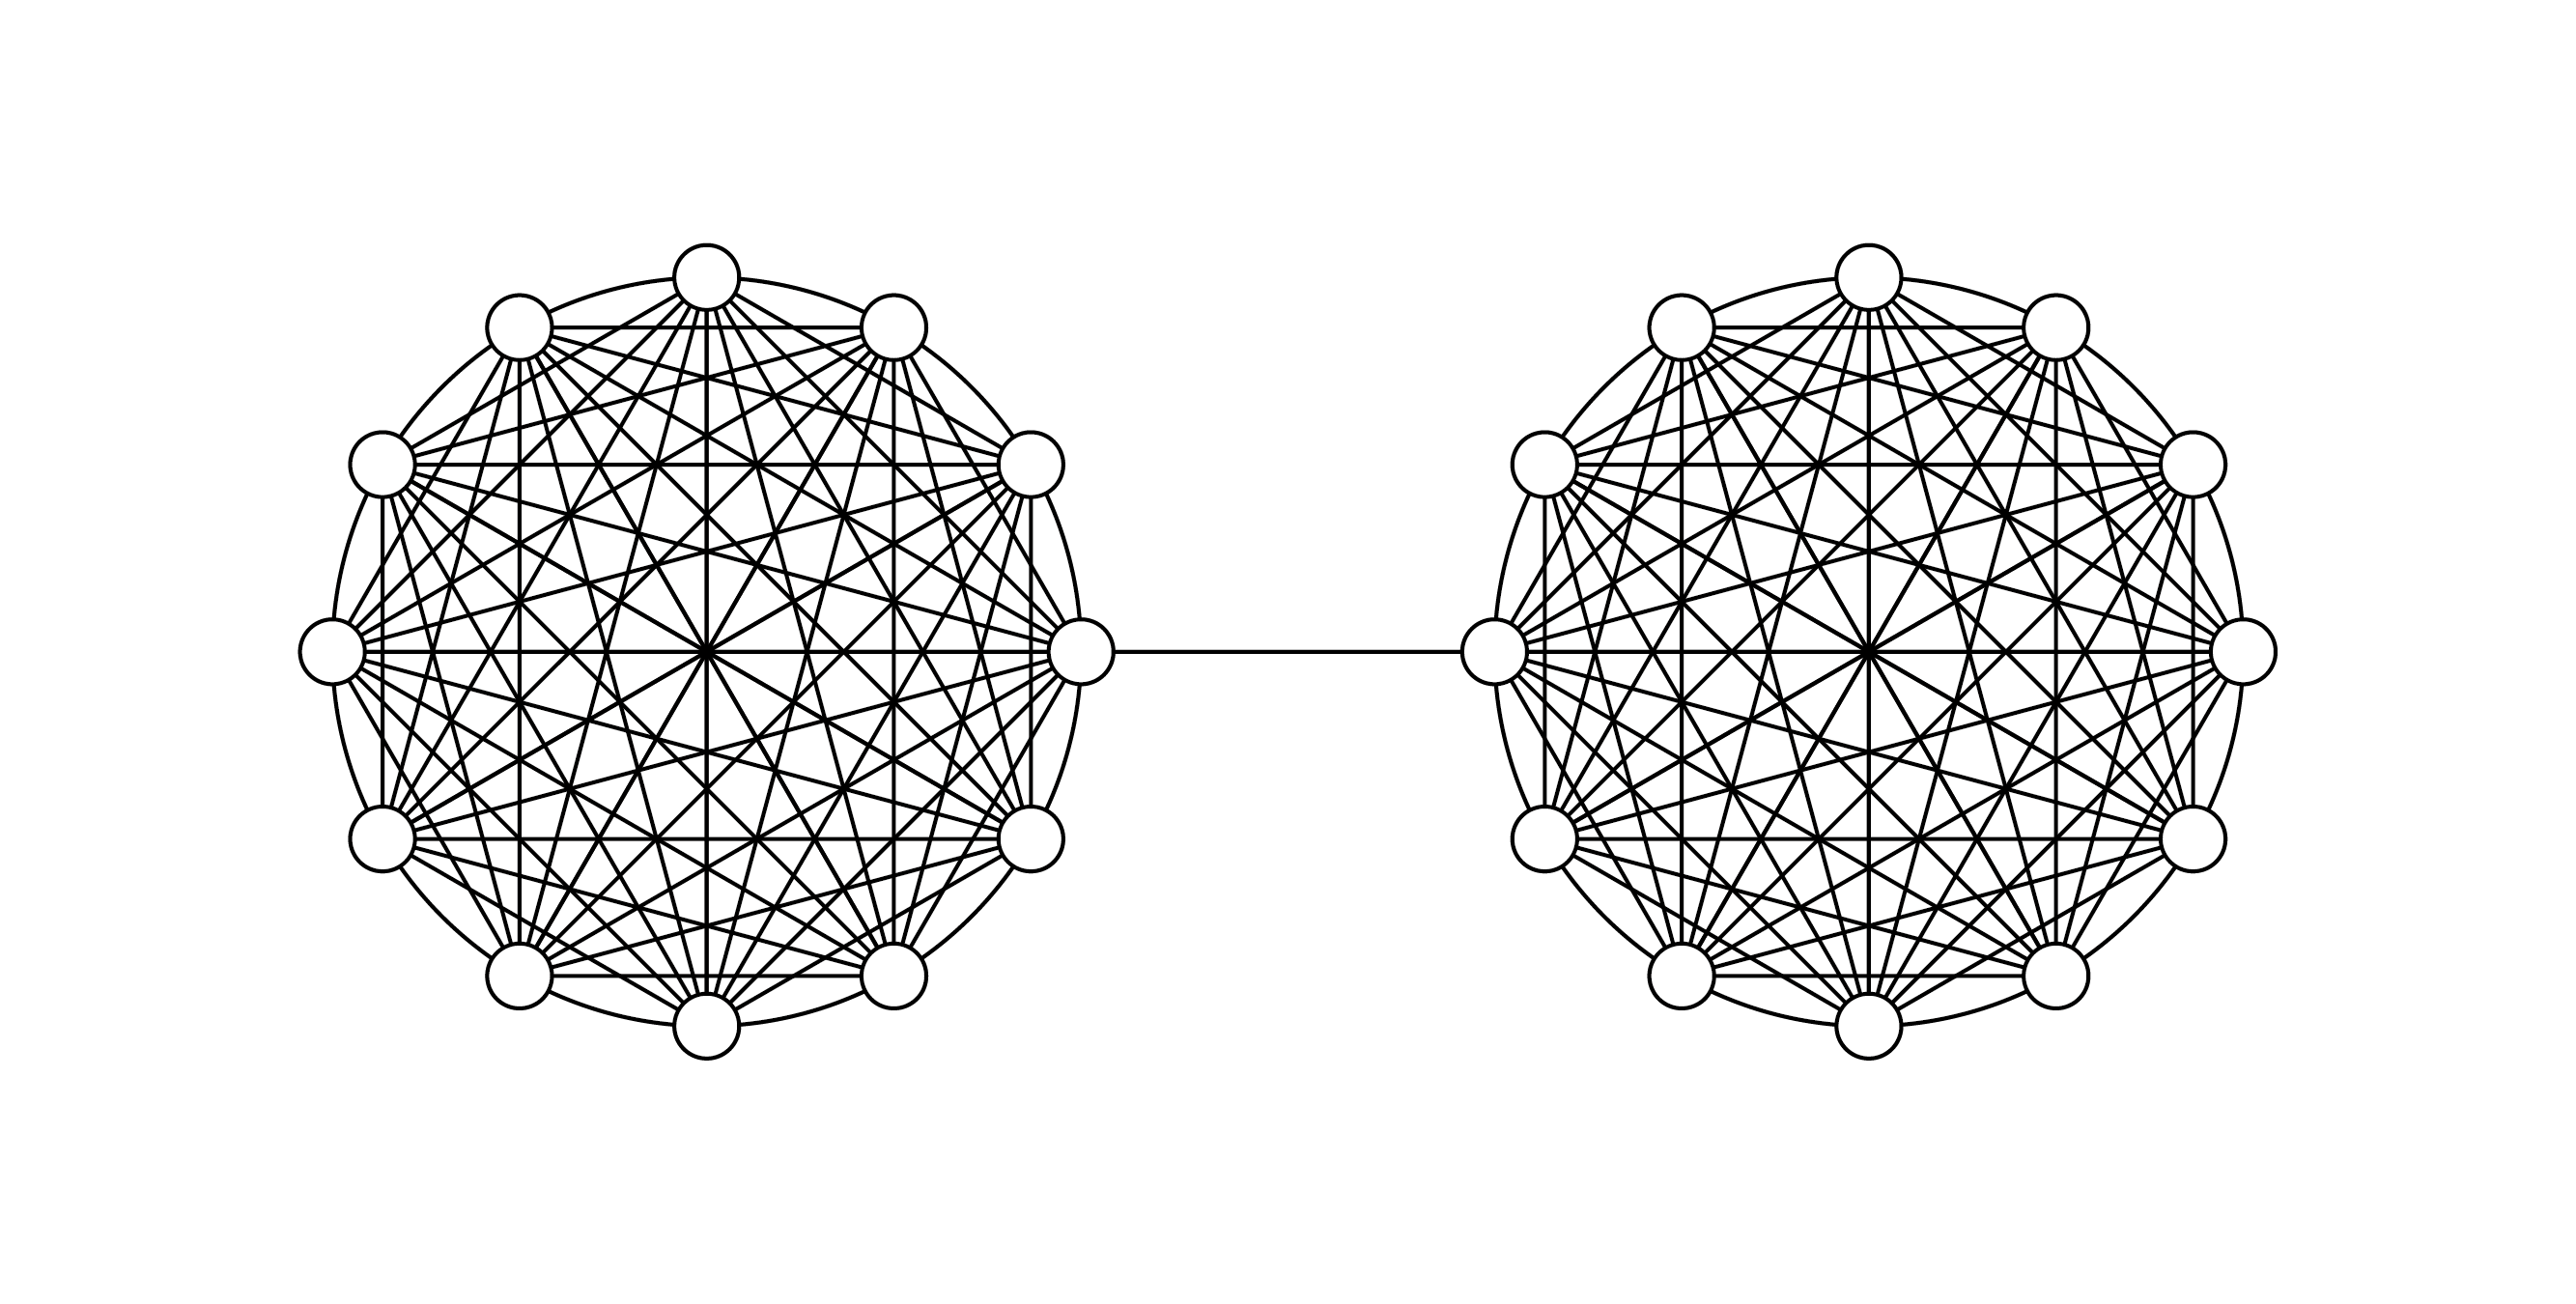
\includegraphics[width=0.9\textwidth]{images/dumbbell_graph.png}
    \caption{An example of a dumbbell graph.\label{dumbbell_graph}}
  \end{figure}

\end{definition}

It is not hard to see that $\Phi = \Theta(1 / n^2)$, where $|V| = 2n$: simply
cut along the edge connecting the complete graphs. By Cheeger's inequality, it
follows that $\nu_2 \le \Theta(1 / n^2)$.

We wish to show that this is a tight bound, ie. $\nu_2 = \Omega(1 / n^2)$.
Intuitively, this is true, because we know from the main result of last week
that the number of lazy random walk steps $t$ it takes to be close to the
stationary distribution is directly proportional to $1 / \nu_2$. 

Indeed, there is probability $1 / n$ to get to the spectral vertex (the vertex
connecting the two complete graphs), and from the spectral vertex, there is
probability $1 / n$ chance to cross to the other $K_n$. But let's do this
rigorously.

\begin{lemma}
  Let $G = (V, E)$, $u, v \in V$. Suppose there exists a path $P(u, v)$ from $u$
  to $v$ with length $3$, as demonstrated in Figure \ref{path_example}. (Note
  that $(u, v)$ need not be an edge in $G$.) Let $L_{u, v}$ be the Laplacian of
  the $(u, v)$-line graph, and $L_{P(u, v)}$ be the Laplacian of the $P(u,
  v)$-path graph.

  \begin{figure}
    \centering
    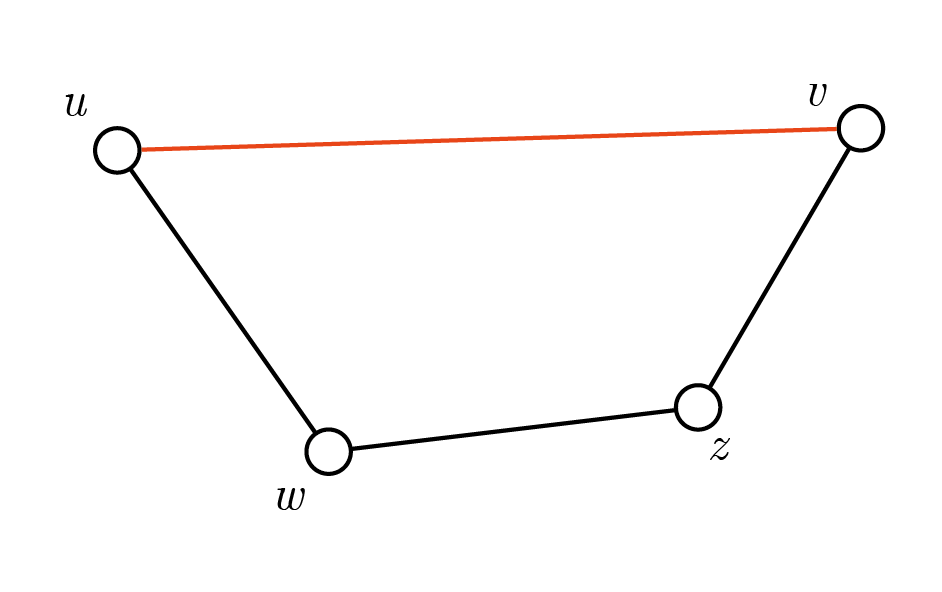
\includegraphics[width=0.5\textwidth]{images/path_example.png}
    \caption{$P(u, v)$ is a path of length $3$ via $(u, w, z,
      v)$.\label{path_example}}
  \end{figure}

  Then 

  \[ (\ones_u - \ones_v)(\ones_u - \ones_v)^{\top} = L_{u, v} \preceq 3 L_{P(u,
  v)} \]
\end{lemma}

\begin{proof}
  By Cauchy-Schwarz,

  \begin{align*}
    ((x_u - x_w) + (x_w - x_z) + (x_z - x_v))^2 &\le 3 ((x_u - x_w)^2 +
    (x_w - x_z)^2 + (x_z - x_v)^2) \qquad &\forall x \\
    (x_u - x_v)^2 &\le 3 ((x_u - x_w)^2 + (x_w - x_z)^2 + (x_z - x_v)^2) \qquad
    &\forall x \\
    L_{u, v} &\preceq 3 (L_{u, w} + L_{w, z} + L_{z, v}) = 3 L_{P(u, v)}
  \end{align*}
\end{proof}

The following is a useful lemma that establishes a lower bound on $\nu_2$
given $\lambda_2$ (and the maximum degree of a graph, $d_{\max}$).
\begin{lemma}
  \[ \nu_2 \ge \frac{\lambda_2}{d_{\max}}. \]
\end{lemma}

\begin{proof}
  Recall by Courant-Fischer,

  \begin{align*}
  \nu_2 &= \min_{\V{x}^{\top} (\V{D}^{1/2} \ones) = 0}
  \frac{\V{x^{\top} N x}}{\V{x^{\top} x}} = \min_{\substack{T \subset \rea^V\\
  \dim(T) = 2}} \max_{x \in T} \frac{\V{x^{\top} N x}}{\V{x^{\top} x}} \\
  \intertext{We can substitute $x = D^{1/2} y$. Since $x \in T$, it follows that
  $y \in \V{D}^{1/2} T$:}
  &= \min_{\substack{T \subset \rea^V\\ \dim(T) = 2}} \max_{y \in \V{D}^{1/2} T}
  \frac{\V{y^{\top} L y}}{\V{y^{\top} D y}} \\
  \intertext{Let $\hat{T} = \V{D}^{1/2} T$. Note that we can assume that $\V{D}$ is one-to-one and
  onto, and hence $\dim(\hat{T}) = 2$. Otherwise, one of the vertices
    has degree zero, and hence $\lambda_2 = 0.$ Thus,}
  &= \min_{\substack{\hat{T} \subset \rea^V\\ \dim(\hat{T}) = 2}} \max_{y \in \hat{T}} \frac{\V{y^{\top} L y}}{\V{y^{\top} D y}} \\
  &\ge \min_{\substack{\hat{T} \subset \rea^V\\ \dim(\hat{T}) = 2}} \max_{y \in \hat{T}} \frac{\V{y^{\top} L y}}{d_{\max} \V{y^{\top} y}} \\
  &= \frac{1}{d_{\max}} \min_{\substack{\hat{T} \subset \rea^V\\ \dim(\hat{T}) = 2}} \max_{y \in \hat{T}} \frac{\V{y^{\top} L y}}{\V{y^{\top} y}} \\
  &= \frac{\lambda_2}{d_{\max}}
  \end{align*}
\end{proof}

\begin{theorem} 
  $\nu_2 = \Omega(1 / n^2)$ for a dumbbell graph.
\end{theorem}

\begin{proof}
  We begin by finding a bound on $\lambda_2(L_G)$, then apply the second lemma
  to establish the relationship between $\lambda_2$ and $\nu_2$.

  Observe that for any $u, v \in V$, there is a path $P(u, v)$ from $u$ to
  $v$ of length $3$. Thus, we can apply our first lemma:

  \[ L_{u, v} \preceq 3 L_{P(u, v)} \preceq 3 L_G \]

  where the second $\preceq$ follows because we are simply adding more squares
  to $L_{P(u, v)}$. By summing over all pairs $(u, v) \in V \times V$, $u \neq
  v$, 

  \begin{align*}
    L_{K_{2n}} &\preceq 3 {2n \choose 2} L_G \\
    \intertext{By a corollary of Courant-Fischer, we know that}
    \lambda_2(L_{K_{2n}}) &\le \lambda_2\left( 3 {2n \choose 2} L_G \right) = 3
    {2n \choose 2} \lambda(L_G)
    \intertext{Recall $\lambda_2(L_{K_n}) = n$, so $\lambda_2(L_{K_{2n}}) = 2n$.
    Furthermore, $3 {2n \choose 2} = \Theta(n^2)$. Thus,}
    \lambda_2(L_G) &= \Omega \left( \frac{1}{n} \right)
   \intertext{Applying the second lemma, and the fact that $d_{\max} = n$ for
 the dumbbell graph,}
  \nu_2(L_G) &\ge \frac{\lambda_2(L_G)}{n} = \Omega\left(
  \frac{1}{n^2} \right)
  \end{align*}
\end{proof}

\section{Expanders}

To motivate the following section, we notice that it would be nice to have
graphs that approximate cliques, in the sense that these graphs quickly approach
their stationary distribution but that are also sparser than cliques.

\begin{definition}
  A $d$-regular, unweighted graph $G$ is said to be an
  \textbf{$\varepsilon$-expander} if 

  \begin{align*}
  - \varepsilon d &\le \lambda_i(A) \le \varepsilon d \qquad &\forall i < n. \\
  \intertext{Equivalently, because $L = dI - A$ and $N = \frac{1}{d} L$,}
  (1 - \varepsilon) d &\le \lambda_j(L) \le (1 + \varepsilon) d \qquad &\forall
  j \neq 1 \\
  1 - \varepsilon &\le \lambda_j(N) \le 1 + \varepsilon \qquad &\forall j \neq 1 \\
  (1 - \varepsilon) L_{K_n} &\preceq \frac{n}{d} L_G \preceq (1 + \varepsilon)
  L_{K_n}
  \end{align*}

\end{definition}

The last equivalence is not trivial, so we will demonstrate it below:

\begin{lemma}
  $G$ is a $d$-regular $\varepsilon$-expander iff

  \[ (1 - \varepsilon) L_{K_n} \preceq \frac{n}{d} L_G \preceq (1 + \varepsilon)
  L_{K_n} \]
\end{lemma}

\begin{proof}
  This is equivalent to showing

  \begin{align*}
    (1 - \varepsilon) \V{x^{\top}} \V{L}_{K_n} \V{x} &\le \frac{n}{d}
    \V{x^{\top}} \V{L}_G \V{x} \le (1 + \varepsilon) \V{x^{\top}} \V{L}_{K_n}
    \V{x} &\qquad \forall \V{x} \\
    \intertext{Any $\V{x}$ can be expressed as the linear combination of the
    eigenvectors of $\V{L}_{K_n}$. Thus, $\V{x} = c \V{\ones} + \V{y}$, where
      $\V{y^{\top} \ones} = 0$ and $\V{y}$ has eigenvalue $n$. Restrict the
      inequality we are trying to prove to the space orthogonal to
      $\text{span}\{\ones\}$:}
    (1 - \varepsilon) n \V{y^{\top} y} &\le \frac{n}{d} \V{y^{\top} L_G y}
    \le (1 + \varepsilon) n \V{y^{\top} L_{K_n} y} &\qquad \forall y \\
    (1 - \varepsilon) d \V{y^{\top} y} &\le \V{y^{\top} L_G y} \le (1 +
    \varepsilon) d \V{y^{\top} L_{K_n} y} &\qquad \forall y \\
    (1 - \varepsilon) d &\le \frac{\V{y^{\top} L_G y}}{\V{y^{\top} y}} \le (1 +
    \varepsilon) d &\qquad \forall y \\
  \end{align*}

  which is true by our second definition of the $d$-regular
  $\varepsilon$-expander.
\end{proof}

In particular $d$-regular $\varepsilon$-expanders are nice because it would
otherwise be difficult for such graphs to arise randomly:

Let $\mathcal{G}(n, p)$ be a random graph model with $n$ vertices such that each
edge $(u, v)$ occurs independently with probability $p$.

Then $\av[\text{no. of edges}] = p {n \choose 2}$ and $\av[\text{deg } v] =
(n - 1) p$. In other words, if we want $d_v$ to be constant (to mimic a
$d$-regular graph), we would only need $p \sim \frac{1}{n}$. However, for the
graph to also be connected we would have to take $p \sim \frac{\log n}{n}$.
Therefore, a connected random graph will most likely be more dense than its
$d$-regular counterpart.

\begin{theorem}
  $\forall \varepsilon > 0.\; \exists d(\varepsilon)$ such that there is a
  ``family'' of $d$-regular $\varepsilon$-expanders, ie. an increasingly-sized
  collection of $\varepsilon$-expanders.
\end{theorem}

\begin{corollary}
  Let $G$ be a $d$-regular $\varepsilon$-expander. Then $\nu_2(G) \ge 1 -
  \varepsilon = \Omega(1)$ implies we only need $\Theta(\log n)$ steps to get
  close to stationary, and we only need $\log d$ bits of randomness to choose
  the next vertex.

  Compare this to $K_n$, which also takes $\Theta(\log n)$ steps to get close to
  stationary, but would need $\log n$ bits of randomness to choose the next
  vertex.
\end{corollary}

\end{document}


%%% Local Variables:
%%% mode: latex
%%% TeX-master: t
%%% End:
